\textcolor{red}{AF: one thing is the problem and a different one is the solution, this section seems to talk about the solution, not the problem. A section about the problem should be added,}

\textcolor{red}{AF: a block diagram must be added and referred to.}

\begin{figure*}
	\centering
	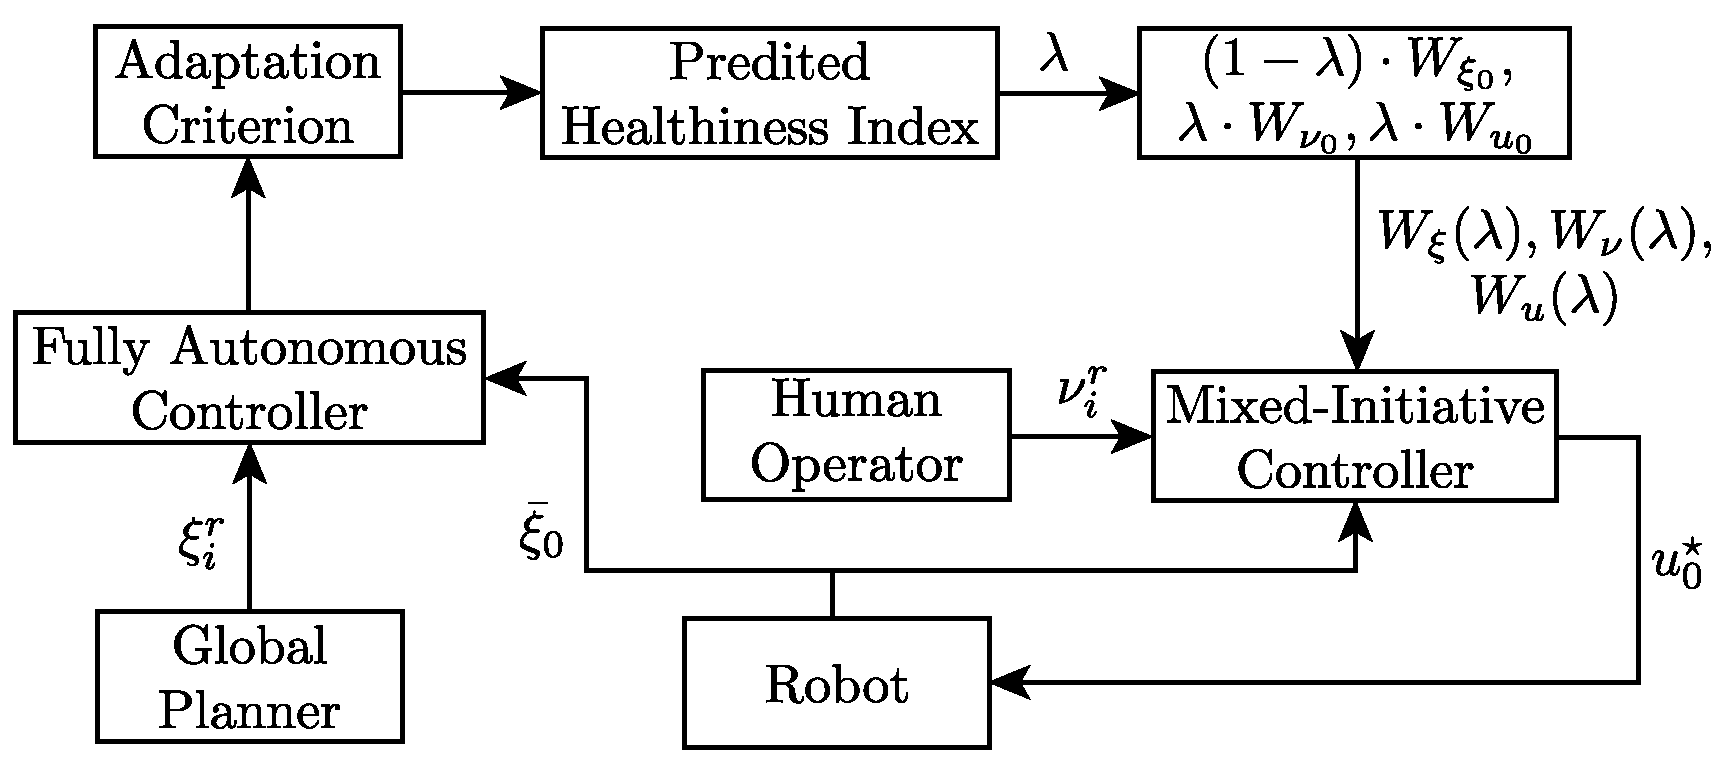
\includegraphics[width=1.0\textwidth]{figure/block_diagram}
\end{figure*}

The base controller of this work is a zone NMPC with trajectory-dependent penalty parameters. The zone NMPC model takes into account the robot dynamics plus part of the robot dynamics that the human is able to control, e.g. attitude and height \textcolor{red}{AF: to be checked}). The controller is driven by the predicted trajectories from another NMPC (namely, low-level NMPC), which considers just the dynamics of the robot. At each time instant, two constrained optimization problems are solved numerically, yielding two different feedback control policies.

In this section, we present the respective prediction models for each NMPC, as well as the nonlinear programs (NLP) arising in each NMPC formulation. 
%%%%%%%%%%%%%%%%%%%%%%%%%%%%%%%%%%%%%%%%%%%%%%%%%%%%%%%%%%%%%%%%%%%%%%%%%%%%%%%%%%%%%%
\subsection{Prediction Models}
Let $\{\mathcal{B}\}$ be the body-fixed frame, located at the center of mass (CoM) of a quadrotor, aligned with the North-West-Up (NWU) inertial frame $\{\mathcal{I}\}$. In order to implement the low-level NMPC, we consider a nonlinear dynamic model of the form
\begin{equation*}
	\dot{\xi} = f_1(\xi,u).
\end{equation*}
We then define the state vector, considering only the dynamics of the robot:
\begin{equation*}
	\xi := (p,\gamma,v_b,\omega,\Omega)^T \in \mathbb{R}^{16},
\end{equation*}
where $ p := (x, y, z)$  is the position vector in $\{\mathcal{I}\}$, $ \gamma := (\phi,\theta,\psi)$ are the Euler angles for orientation, $v_b := (v_x, v_y, v_z)$ is the linear velocities vector in $\{\mathcal{B}\}$, $\omega := (\omega_x, \omega_y, \omega_z)$ is the vector of angular rates, and finally $\Omega := (\Omega_1,\Omega_2,\Omega_3,\Omega_4)$ is the vector containing the rotation speed of the propellers. Hence, we regard the following quadrotor model:
 \begin{equation*}
 	\begin{aligned}
 	\dot{p} &= Rv_b \\
 	\dot{\gamma} &= T \omega\\
	\dot{v}_b &= \frac{1}{m}F - R^{T}G - \omega\times v_b\\
	\dot{\omega} &= J^{-1}(M - \omega\times J\omega)\\
	\dot{\Omega} &= \frac{\tau}{J_m},
 	\end{aligned}%
 \end{equation*}
 \textcolor{red}{AF: what about drag of the rotor in the motor equation?}
where the mass of the quadrotor is $m \in \mathbb{R}^+$, and $G \vcentcolon =(0, 0, mg)^T$ with $g$ being the gravitational acceleration. The robot inertia matrix with respect to its CoM and expressed in $\{\mathcal{B}\}$ is given by $J \vcentcolon = \text{diag}(J_{xx}, J_{yy}, J_{zz}) \in \mathbb{R}^{3 \times 3}$. The rotation matrix from  $\{\mathcal{B}\}$ to $\{\mathcal{I}\}$ is expressed as $R \in SO(3)$. The matrix $T \vcentcolon \mathbb{R}^3 \rightarrow \mathbb{R}^{3 \times 3}$ represents the relation between the instantaneous rates of change of the Euler angles and the instantaneous components of $\omega$. \textcolor{red}{AF: define ALL the symbols introduced, here and after} The total external forces and moments applied to the CoM of quadrotor in $\{\mathcal{B}\}$ are defined as 
 \begin{equation}
 	\begin{aligned}
    F & \vcentcolon =  \sum_{i=1}^4 C_T\Omega_{i}^2\mathbf{1}_z, \quad M \vcentcolon = (M_x, M_y, M_z)^T
	\end{aligned}
 \end{equation}\label{eq:force_moments}
 with
 \begin{equation*}
 	\begin{aligned}
    M_x &= C_T\cdot l(-\Omega_{1}^{2}-\Omega_{2}^{2}+\Omega_{3}^{2}+\Omega_{4}^{2}),\\
    M_y &= C_T\cdot l(-\Omega_{1}^{2}+\Omega_{2}^{2}+\Omega_{3}^{2}-\Omega_{4}^{2}),\\
    M_z &= C_D(-\Omega_{1}^{2}+\Omega_{2}^{2}-\Omega_{3}^{2}+\Omega_{4}^{2}),
 	\end{aligned}
 \end{equation*}
where $C_T$ is the thrust coefficient, $C_D$ is the drag coefficient, and $l$ is half of the distance between motors. When considering a medium-size quadrotor, the rotor inertia $J_m$ is not negligible as the radius of the rotor's axle is not small. Therefore, we consider the rotor torques as the control inputs of this system
\begin{equation}
	u := (\tau_1,\tau_2,\tau_3,\tau_4)^T \in \mathbb{R}^4.\label{eq:control_inputs}
\end{equation}



Moreover, for the zone NMPC let us consider the following nonlinear dynamic model:
\begin{equation*}
	\dot{\sigma} = f_2(\sigma,u).
\end{equation*}
This model is composed of the robot dynamics plus part of the robot dynamics that the human is able to control. For a quadrotor, the latter is essentially composed of the rotational dynamics and the translational dynamics in $z$ (which is directly linked to the collective speed of the propellers). Thus, we can formally define the part of the dynamics controlled by the human as:
\begin{equation*}
	\nu \vcentcolon = (\gamma, \omega, \Omega)^T \in \mathbb{R}^{10}.
\end{equation*}
Then, the state vector of the zone NMPC can be characterized as follows:
\begin{equation*}
	\sigma \vcentcolon = (p,\gamma,v_b,\omega,\Omega,\nu)^T \in \mathbb{R}^{26},
\end{equation*}
while the control inputs are the rotor torques, likewise regarded in \eqref{eq:control_inputs}.



\textcolor{red}{AF: this is confusing. Some of the states seem to appear twice. I would rather say that in this controller there are some additional exogenous inputs provided by the human which are the desired orientation and desired total thrust and give to these quantities a different name. In any case these quantities should not appear in the state of the robot, in the sense that they do not affect the robot dynamics directly, but rather in the objective function, i.e., in the controlled (closed loop) dynamics, in the same way the desired trajectory appear.}


%%%%%%%%%%%%%%%%%%%%%%%%%%%%%%%%%%%%%%%%%%%%%%%%%%%%%%%%%%%%%%%%%%%%%%%%%%%%%%%%%%%%%%
\subsection{Nonlinear Programs}
We regard the nonlinear program (\textbf{NLP$_1$}) corresponding to the constrained optimization problem of the low-level NMPC as follows:
\begin{equation*}\label{eq:nlp1}
{\!\!\!\!\!}{\!\!}\begin{aligned}
&\underset{\begin{subarray}{c}
\xi_0, \dots, \xi_N, \\
u_0, \dots, u_{N-1}
\end{subarray}}{\min}	    &&\frac{1}{2}\sum_{i=0}^{N-1} \|\eta(\xi_i, u_i)-\Bar{\eta}\|^2_{W} + \frac{1}{2}\|\eta_N(\xi_N)- \Bar{\eta}_N\|^2_{W_N}\\ 
&\,\,\,\quad \text{s.t.}    &&\xi_0 = \Bar{\xi}_0, \\
& 						    &&\xi_{i+1} - F_1(\xi_i,u_i) = 0, \,\,\,\,\,\, i = 0,\dots, N-1,\\
& 						    &&\Omega_i\in \mathbb{E}, \,\,\,\,\,\,\,\,\,\,\,\,\,\,\,\,\,\,\,\,\,\,\,\,\,\,\,\,\,\,\,\,\,\,\,\,\,\,\,\,\, i = 0,\dots, N-1,\\
& 						    &&u_i\in \mathbb{U}, \,\,\,\,\,\,\,\,\,\,\,\,\,\,\,\,\,\,\,\,\,\,\,\,\,\,\,\,\,\,\,\,\,\,\,\,\,\,\,\,\,\, i = 0,\dots, N-1,
\end{aligned}{\!\!\!}
\end{equation*}
\textcolor{red}{AF: shouldn't the desired state $\Bar{\eta}$ depend on $i$ since it is time varying? Also please make it clear from the beginning, in the problem setting, that this is a trajectory that is passed to the system by an external planner in order to execute the task.}
where $\xi \in \mathbb{R}^{n_{\xi}}$ and $u \in \mathbb{R}^{n_u}$ denote the state and input trajectories of the discrete-time robot system whose dynamics are described by $F_1 \vcentcolon \mathbb{R}^{n_{\xi}} \times \mathbb{R}^{n_u} \rightarrow \mathbb{R}^{n_{\xi}}$. The residuals in the stage and terminal least-squares terms are denoted by $\eta \vcentcolon \mathbb{R}^{n_{\xi}} \times \mathbb{R}^{n_u} \rightarrow \mathbb{R}$ and $\eta_N \vcentcolon \mathbb{R}^{n_{\xi}} \rightarrow \mathbb{R}$, and will be penalized by the symmetric positive-definite matrices $W$ and $W_N$, respectively. The output variables $\Bar{\eta} \vcentcolon \mathbb{R}^{n_{\xi}} \times \mathbb{R}^{n_u} \rightarrow \mathbb{R}$ and $\Bar{\eta}_N \vcentcolon \mathbb{R}^{n_{\xi}} \rightarrow \mathbb{R}$ represent the time-varying references passed to the automatic controller. We denote the admissible sets of $u$ and $\Omega$ as $\mathbb{U} \vcentcolon = [\ubar{u}, \Bar{u}]$ and $\mathbb{E} \vcentcolon = [\ubar{\Omega}, \Bar{\Omega}]$, where the bounds $\ubar{u}$, $\Bar{u}$, $\ubar{\Omega}$, and $\Bar{\Omega}$ are given. Finally, $N$ and $\Bar{\xi}_0$ denote the horizon length and the current state of the system, respectively. 

\textcolor{red}{AF: Another general comment I have is that I am not sure that making the difference between Euler angles is mathematically correct, anyway let's go back to this later.}

Similarly, the nonlinear program (\textbf{NLP$_2$}) that corresponds to the constrained optimization problem of the zone NMPC is:
\begin{equation*}\label{eq:nlp2}
{\!\!\!\!\!}{\!\!}\begin{aligned}
&\underset{\begin{subarray}{c}
\sigma_0, \dots, \sigma_N, \\
u_0, \dots, u_{N-1}
\end{subarray}}{\min}	    &&\frac{1}{2}\sum_{i=0}^{N-1} \|\eta(\sigma_i,u_i)-\Tilde{\eta}\|^2_{W(\epsilon_i^ \star)} + \frac{1}{2}\|\eta_N(\sigma_N)-\Tilde{\eta}_N\|^2_{W_N(\epsilon_i^\star)}\\ 
&\,\,\,\quad \text{s.t.}    &&\sigma_0 = \Bar{\sigma}_0, \\
& 						    &&\sigma_{i+1} - F_2(\sigma_i,u_i) = 0, \,\,\,\,\,\, i = 0,\dots, N-1,\\
& 						    &&\Omega_i\in \mathbb{E}, \,\,\,\,\,\,\,\,\,\,\,\,\,\,\,\,\,\,\,\,\,\,\,\,\,\,\,\,\,\,\,\,\,\,\,\,\,\,\,\,\,\,\, i = 0,\dots, N-1,\\
& 						    &&u_i\in \mathbb{U}, \,\,\,\,\,\,\,\,\,\,\,\,\,\,\,\,\,\,\,\,\,\,\,\,\,\,\,\,\,\,\,\,\,\,\,\,\,\,\,\,\,\,\,\, i = 0,\dots, N-1,
\end{aligned}{\!\!\!}
\end{equation*}

\textcolor{red}{AF: OK, now I think understand better why you are elongating the state vector $\xi$ in $\eta$ repeating some its entries again, I guess this is in order to make the difference in the cost function and then the weighting matrix will take care of the mixing, giving more importance to $\xi$ part of $\eta$ or to the repeated entries. I think this should be better explained. I think that it is probably better to separate the two parts of the norms, the trajectory following and the human-following one, otherwise it remains hidden in the formulation for the reader and it could be misunderstood. I think it is better to not introduce $\eta$ as an extended/repeated $\xi$ but to actually reuse $\xi$ in this second optimization problem together with a portion of $\xi$ which you can call $\xi_h$ and is  the human 'output' to be regulated in order to match the human 'commands' and to show them separately in this optimization. In this way everything becomes more clear in my view. Another way to do so is to immediately define block-diag  structure of the weighting matrix and to define the vector $\eta$ as the stack of $\xi$ and $\xi_h$ so that is more clear.}

\textcolor{red}{AF: another thing that is confusing at this point is how come the human can give desired propeller rates for each propeller at the same time, together with the desired attitude? This is too  complex for a human. What the human specifies is actually the total thrust, which is a function of the propeller rates but it does not specify them completely, there are several DoF left. We have to immediately say how we go from the desired thrust to all the propeller rates. I guess this partially explained in the appendix, but on the one side the explanation given in appendix is not completely clear to me and on the other side I think it should be immediately explained, not delayed to the appendix. }

where $\sigma \in \mathbb{R}^{n_{\sigma}}$ and $u \in \mathbb{R}^{n_u}$ denote the state and input trajectories of the discrete-time robot-human system whose dynamics are described by $F_2 \vcentcolon \mathbb{R}^{n_{\sigma}} \times \mathbb{R}^{n_u} \rightarrow \mathbb{R}^{n_{\sigma}}$. The residuals in the stage and terminal least-squares terms are denoted by $\eta \vcentcolon \mathbb{R}^{n_{\sigma}} \times \mathbb{R}^{n_u} \rightarrow \mathbb{R}$ and $\eta_N \vcentcolon \mathbb{R}^{n_{\sigma}} \rightarrow \mathbb{R}$, and will be penalized by the time-varying matrices $W(\epsilon_i^\star), {W}_N(\epsilon_i^\star) \succ 0$, respectively. The output variables $\Tilde{\eta} \vcentcolon \mathbb{R}^{n_{\sigma}} \times \mathbb{R}^{n_u} \rightarrow \mathbb{R}$ and $\Tilde{\eta}_N \vcentcolon \mathbb{R}^{n_{\sigma}} \rightarrow \mathbb{R}$ represent the time-varying references coming from both global planner (offline) and human inputs (online). Notice that $W(\epsilon_i^\star)$ and ${W}_N(\epsilon_i^\star)$ depend on the predicted Euclidean distance ($\epsilon^\star_i$), which we will introduce in the next section, using the prediction model in the low-level NMPC. Accounting for reciprocal feasibility between controllers, the remaining constraints in (\textbf{NLP$_2$}) are kept the same as in (\textbf{NLP$_1$}). 
%%%%%%%%%%%%%%%%%%%%%%%%%%%%%%%%%%%%%%%%%%%%%%%%%%%%%%%%%%%%%%%%%%%%%%%%%%%%%%%%%%%%%%